%%%%%%%%%%%%%%%%%%%%%%%%%%%%%%%%%%%%%%%%%%%%%%%%%%%%%%%%
%%%%                                              %%%%%%
%%%%  Author: Peter Wilson                        %%%%%%
%%%%                                              %%%%%%
%%%%  Non-linear analysis background
%%%%                                              %%%%%%
%%%%%%%%%%%%%%%%%%%%%%%%%%%%%%%%%%%%%%%%%%%%%%%%%%%%%%%%


%fref generates automatically the respective abreviation/word in the text for the reference. You just have to define a label starting with the respective keyword.
%english: chap, sec, fig, eq, app
%deutsch: chap/kap, abs, abb, gl, anh
%see http://ctan.space-pro.be/tex-archive/macros/latex/contrib/fancyref/fancyref.pdf for more \section

%\onehalfspacing
%\setlength{\belowcaptionskip}{-17pt}

\chapter{Non-linear analysis background - revised 1}
\label{chap:chapter_2_2}

\renewcommand{\Thema}{Non-linear analysis background}

\lettrine[lines=2]{T}{he} expedient practical design of engineering structures is often considered fulfilled after the confirmation of allowable deflections and stresses throughout the entire domain. Although the design may in fact be adequate in the vast majority of cases, structural stability is an oft overlooked phenomena in "bread and butter" engineering analysis and is by no means guaranteed by acceptable displacements and stresses. Indeed, some of the most catastrophic structural failures such as the Tacoma Narrows Bridge (1940) and the Twin Towers (2001) have root  causes stemming from system instability and reinforce the importance of stability analysis.

Structural stability, expressed crudely, can be thought of as "the power to recover equilibrium", or, alternatively, a structure can be thought stable at an equilibrium position if it returns to that position following a temporary perturbation \cite{FelippaStabilityBasics2016}. In terms more relatable, it's clear a person standing on one foot is more susceptible to falling over in the presence of a strong wind than someone firmly planted with both feet. Although the person with both feet planted may sway and bob, they more likely to return to their original equilibrium position after the wind has subsided, that is, they are more stable. In an engineering context, perhaps the most well known stability problem is a long beam subject to a compressive end load: the classic Euler buckling cases. At low load levels the beam will undergo small deformations and trace back to it's original configuration after unloading, however, after the critical Euler buckling load is surpassed structural stability is lost giving way to large arbitrary deformations with non-coincident loading and unloading paths. Although these two simple examples provide a phenomenological picture of structural stability, a more precise engineering description of stability is required for general computational mechanics.

\section{Response diagrams}
Essential to the understanding of structural stability and non-linear FEM is the concept of an equilibrium path, often plotted on load-deflection response diagrams. These diagrams are commonly two dimensional x-y diagrams that plot a representative force quantity against a characterising displacement thereby ascertaining the behaviour of the structure \cite{FelippaNFEMTour2016}.

\begin{figure}[H]
	\centering
	\def\svgwidth{\columnwidth}
	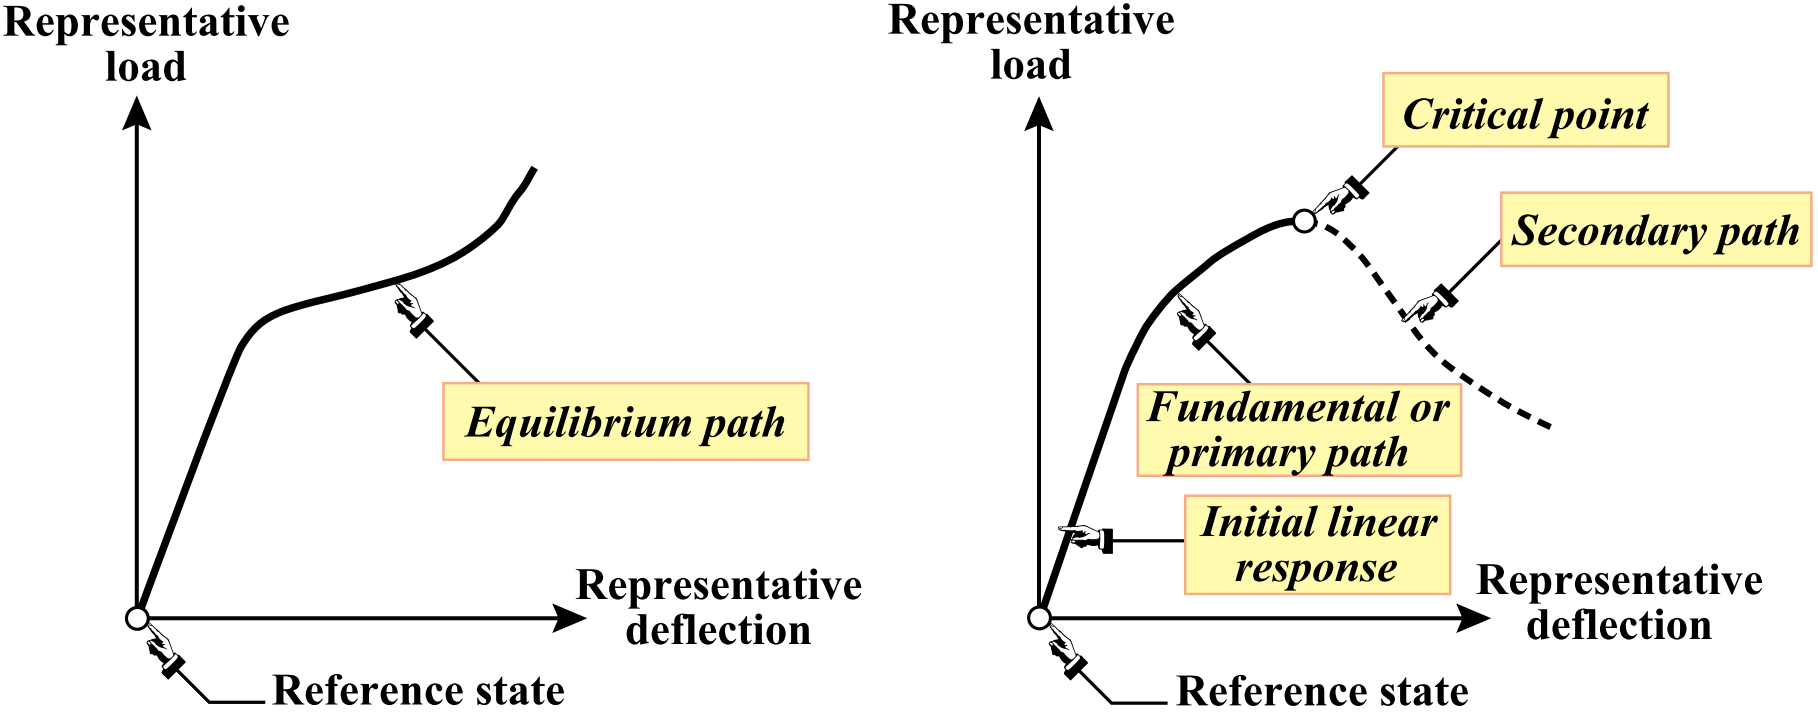
\includegraphics[width=12cm]{images/stability_response_diagram.png}
	\caption{Examples of response diagrams \cite{FelippaNFEMTour2016}}
	\label{stab0}
\end{figure}

The equilibrium path of a response diagram indicates the points in load-deflection space where the structure is in equilibrium, that is, the residual vector $\mathbf{r}$ of the system vanishes. If the scope of structures considered is limited to static linear elastic structures subject to conservative loading characterised by a load factor $\lambda$ linearly scaling the external load vector $\mathbf{f}$, the residual itself is defined as the gradient of the structure's energy $\Pi$ \cite{FelippaNFEMCrit2016}:

\begin{equation}
\mathbf{r}(\mathbf{u},\lambda) = \frac{\partial \Pi (\mathbf{u},\lambda)}{\partial \mathbf{u}}
\label{eqstab0}
\end{equation}

The tangent stiffness matrix of the system is intuitively the slope of the equilibrium path, or alternatively, the Hessian of the structure's energy:

\begin{equation} 
\mathbf{K} = 
\frac{\partial \mathbf{r} (\mathbf{u},\lambda)}{\partial \mathbf{u}} = 
\frac{\partial^2 \Pi (\mathbf{u},\lambda)}{\partial \mathbf{u}\partial \mathbf{u}}
\label{eqstab01}
\end{equation}

Recalling that the equilibrium path of a structure is defined by a vanishing residual, it can be presented in a variety of forms:

\begin{equation} 
\mathbf{r}(\mathbf{u},\lambda) = 
\frac{\partial \Pi (\mathbf{u},\lambda)}{\partial \mathbf{u}} =
\mathbf{K}(\mathbf{u},\lambda) \mathbf{u} - \mathbf{f}(\mathbf{u},\lambda) =
0
\label{eqstab02}
\end{equation}

The above expansion offers a variety of perspectives in which to interpret the equilibrium path. A nod to virtual work methods via variation of system energy is present as well as a simple re-arrangement of the well known $\mathbf{Ku} = \mathbf{f}$ introduced in Bachelor FEM courses.

\section{Stability criterion}
 If the aforementioned Euler beam buckling example is fully derived, it is apparent that the well known Euler critical load formulae precipitate by setting the determinant of the respective system stiffness matrices to zero. In general, loss of structural stability only occurs at critical points $(\mathbf{u}_c,\lambda_c)$ where the determinant of the tangent stiffness matrix vanishes:
 
 \begin{equation} 
 det\big[\mathbf{K}(\mathbf{u}_c,\lambda_c)\big] = 0
 \label{eqstab1}
 \end{equation}
 
 In this Euler case, the instability is manifested by way of bifurcation, commonly referred to as buckling. Bifurcation points designate a critical point in the load-displacement space of the structure where two or more equilibrium paths meet. At these points structure may unpredictably switch equilibrium paths physically manifesting itself as dramatic large deflections. Indeed, in the buckling of a circular-sectioned beam, the direction of buckling deformation is entirely unpredictable (bar coaxing imperfections) with many equilibrium paths coincident at the bifurcation point. Limit, or snap-through, points are the other type of instability that may occur at critical points. In this regime, the critical point coincides with a minimum, maximum or inflection of the load parameter $\lambda$. For an everyday example of snap-through, one can consider an umbrella suddenly inverting in a strong storm, demonstrating that once the snapping wind load is reached predictably large deformations are subsequently observed. 
 
 In the scope of this work the load magnitude that introduces system instability is of key interest, details regarding how to mathematically distinguish between limit and bifurcation points once a critical point has been identified fall outside the domain surveyed. 
 
 The following figure \ref{stab1}(a) illustrates the nature of both instability types on a load-deflection diagram.

\begin{figure}[H]
	\subfloat[Critical points of a response diagram]
	{\label{ref_label2}
		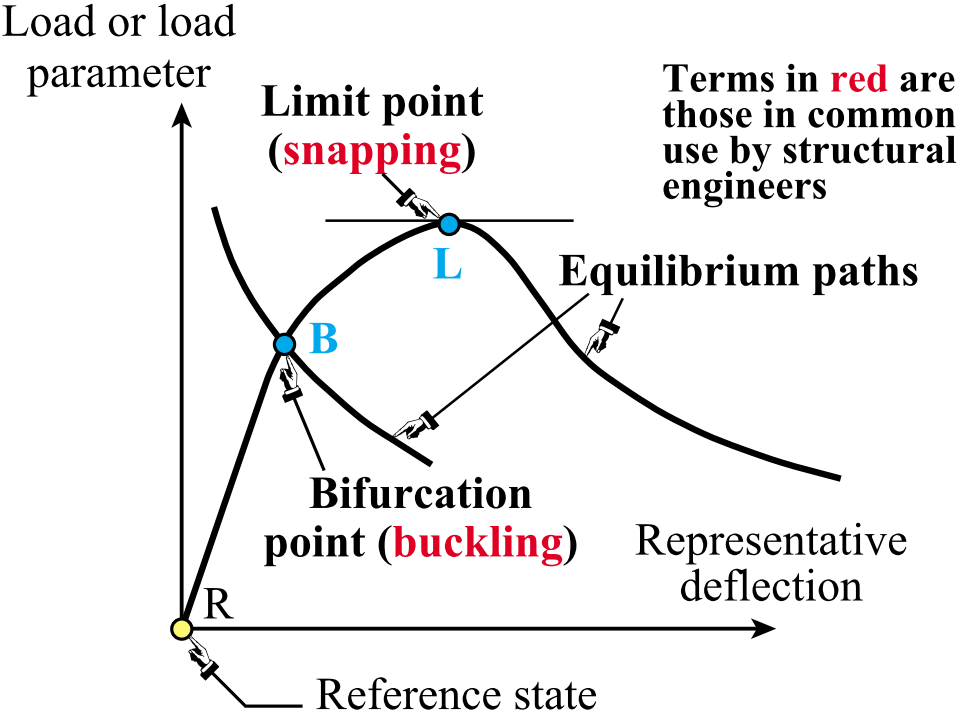
\includegraphics[width=7.3cm]
		{images/stability_eq_path.png}}
	\subfloat[Bifurcation-driven structure critical load]
	{\label{ref_label2}
		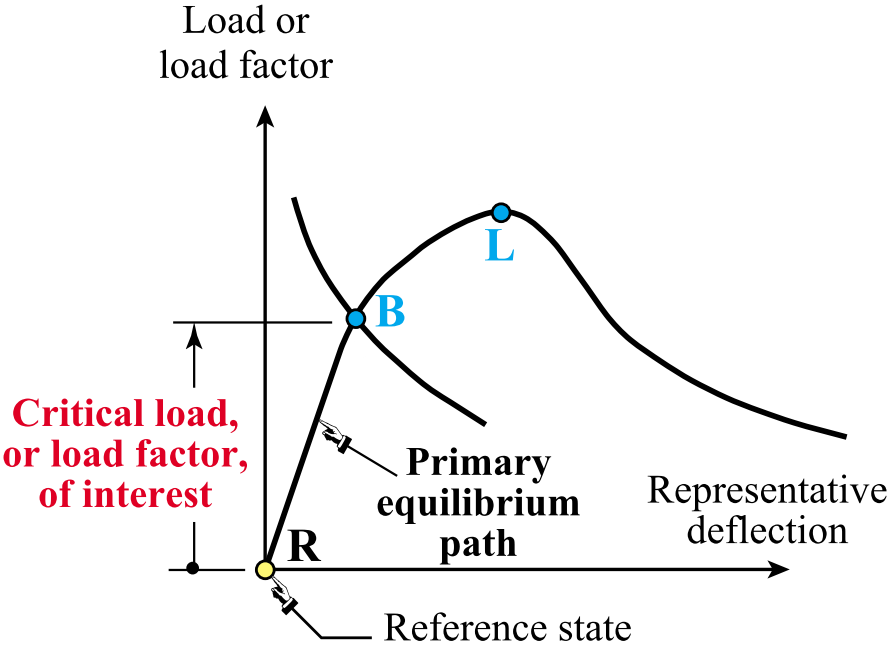
\includegraphics[width=7.3cm]
		{images/stability_buckling.png}}
	\caption{\label{stab1}Stability analysis response diagrams \cite{FelippaStabilityBasics2016}}
\end{figure}

It's clear that after both critical points, as depicted in figure \ref{stab1}(a), the structure looses a significant proportion of it's stiffness indicated by the reduced load required for continual increases of deflection. In this post-buckling state the original function, and indeed safety, of the structure (for example, a roof or building) is likely to be significantly compromised. If such a structural critical point exists at a load level less than the design load cases considered for allowable deflections and stresses then the structure cannot be regarded as properly engineered. Figure \ref{stab1}(b) indicates the critical stability load of the structure, which is the load corresponding to the first critical point on the response diagram. Another, more stringent, approach is to determine the lowest load factor throughout the whole equilibrium path, including the post-critical regime, and take this as the critical stability load.

Despite the need for stability analysis to be regularly considered throughout engineering design, the effort and level of analysis required is clearly quite significant for even simple systems. As such, a linearised approach termed Linear Prebuckling analysis, is often employed.

\section{Linear Prebuckling analysis}
Linear Prebuckling (LPB) analysis offers insight, albeit reduced, into the stability characteristics of structures at a fraction of the computational expense required for a full non-linear equilibrium path analysis.

In order to further interrogate the nature of structural stability, and how it may be simplified, the tangent stiffness matrix in equation \ref{eqstab1} can be decomposed. The total tangent matrix is made up of the material stiffness matrix $\mathbf{K}_m$ (itself composed of the elastic stiffness $\mathbf{K}_e$ and initial displacement stiffness $\mathbf{K}_u$) and the geometric stiffness matrix $\mathbf{K}_g$. Thus equation \ref{eqstab1} can be expanded accordingly:

\begin{equation} 
det\big[
\mathbf{K}_e +
\mathbf{K}_u(\mathbf{u}_0) +
\mathbf{K}_g(\mathbf{u}_c,\lambda_c)
\big] = 
det\big[
\mathbf{K}_m +
\mathbf{K}_g(\mathbf{u}_c,\lambda_c)
\big] = 0
\label{eqstab2}
\end{equation}

It's apparent the expression can be characterized as an eigenvalue problem, thus the eigenvector $\mathbf{z} \neq \mathbf{0}$ corresponding to bifurcation mode shapes can be introduced:

\begin{equation} 
det\big[
\mathbf{K}_m +
\mathbf{K}_g(\mathbf{u}_c,\lambda_c)
\big]\mathbf{z} = 0
\label{eqstab3}
\end{equation}

The non-linear eigenvalue problem can be presented in a linearised form:

\begin{equation} 
det\big[
\mathbf{K}_m +
\hat{\lambda}
\mathbf{K}_g(\mathbf{u}_i,\lambda_i)
\big]\mathbf{z} = 0
\label{eqstab4}
\end{equation}

Equations \ref{eqstab3} and \ref{eqstab4} are identical if $\hat{\lambda}
 = 1,\ \lambda_i = \lambda_c$ and $u_i = u_c$.
 
 If the structure under analysis is considered suitably stiff, with approximately infinitesimal displacements $\mathbf{u} \approx \mathbf{0}$ in the pre-buckling regime and negligible effects of initial displacements ($\mathbf{K}_u(\mathbf{u} \approx \mathbf{0}) \approx \mathbf{0}$), then a simplified stability eigen-problem can be presented:
 
 \begin{equation} 
 det\big[
 \mathbf{K}_e +
{\lambda}
 \mathbf{K}_g(\lambda_{ref})
 \big]\mathbf{z} = 0
 \label{eqstab5}
 \end{equation}
 
 The LPB equation above relies on the additional assumptions that the structure remains linearly elastic until buckling and the structure and loading have no imperfections \cite{FelippaStabilityBasics2016}. It's also clear that the geometric stiffness matrix is assumed to scale proportionally with the load factor, which further relies on the assumption of a linearly elastic structure. Along with these assumptions, LPB analysis is subject to some notable limitations. The first of which is the typical over-estimation of the true stability limit, with accuracy deteriorating as the pre-critical structural behaviour exhibits more non-linearity. Secondly, LPB analysis is unable to distinguish between bifurcation and limit points, with all critical points transformed into bifurcation points. A consequence of this is that the recovered eigenvector associated with a limit point reported as a bifurcation point will be erroneous.
 
 Despite the large swathe of assumptions and limitations accompanying LPB, it is no doubt a sensible and computationally-efficient approach when applied to suitably stiff linear elastic structures, which indeed include a considerable amount of industrial engineering structures.

\section{Stability analysis example}

To illustrate the various aspects stability analysis, including response diagrams and the differences between non-linear and linear critical point analysis, an example Mises two truss system is considered. The full analysis can be found in Appendix \ref{app:Analytical stability analysis of Mises truss}, with only key results reproduced below. The system under consideration is depicted in the following figure:

\begin{figure}[H]
	\centering
	\def\svgwidth{\columnwidth}
	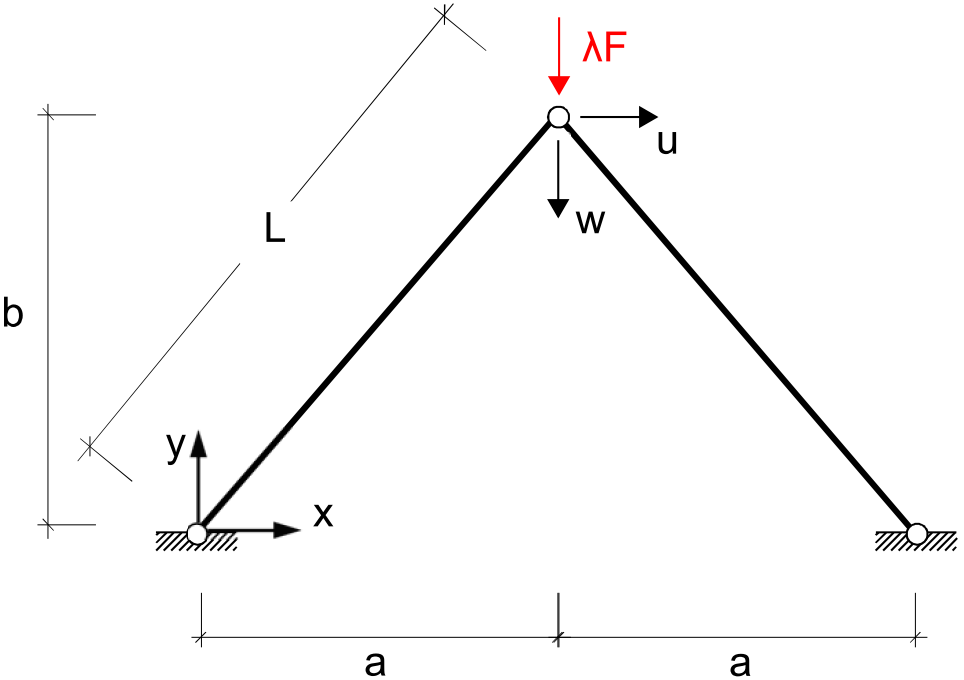
\includegraphics[width=8cm]{images/mises_truss_def.png}
	\caption{Mises truss geometry}
	\label{stab2_1}
\end{figure}

After developing the system's virtual work expression via the 2nd Piola-Kirchhoff stress measure and the conjugate Green-Lagrange strain measure, the residual vector can be expressed as:

\begin{equation} 
\mathbf{r} = 
\begin{pmatrix}
\frac{EA}{L^3} [u^3+uw^2-2bwu+2a^2u] \\
\frac{EA}{L^3} [u^2w + w^3 - 3bw^2 - bu^2 +2b^2w] - \lambda F
\end{pmatrix}
=
\mathbf{0}
\label{eqstab6}
\end{equation}

With the residual vector in hand, the system's stiffness matrix can be expressed as:

\begin{equation} 
\mathbf{K} = 
\frac{\partial \mathbf{r}}{\partial \mathbf{u}}
=
\frac{EA}{L^3}
\begin{pmatrix}
3u^2 + w^2 - 2bw +2a^2 & 2uw -2bu \\
2uw - 2bu & u^2 + 3w^2 - 6bw + 2b^2
\end{pmatrix}
\label{eqstab7}
\end{equation}

Non-linear critical points can be determined by setting the determinant of the stiffness matrix to zero and solving. For the system parameters of ($a=b=EA=F=1$) and under the assumption of $u = 0$ before instability, the non-linear critical points are calculated to be:

 \begin{equation} 
\mathbf{P}_{NL1} = 
 \begin{pmatrix}
 u_{c1} = 0 \\
w_{c1} = 0.4226 \\
\lambda_{c1} = 0.1361
 \end{pmatrix}
 \ ,
 \hspace{10mm}
 \mathbf{P}_{NL2} = 
 \begin{pmatrix}
 u_{c2} = 0 \\
 w_{c2} = 1.5774 \\
 \lambda_{c2} = -0.1361
 \end{pmatrix}
 \label{eqstab8}
 \end{equation}
 
Although the non-linear critical points have been determined, a LPB analysis of the system will be carried out to compare results between the different approaches. As per equation \ref{eqstab5}, a LPB analysis is an eigenvalue problem which, after assuming small displacements and $u=0$ in the pre-buckling regime, reduces to the following expression:

 \begin{equation} 
det
\begin{pmatrix}
\frac{EA}{L^3} 2a^2 - \frac{\lambda F}{b} & 0 \\
0 &  \frac{EA}{L^3} 2b^2 - \frac{\lambda F}{b}
\end{pmatrix}
= 0
\label{eqstab9}
\end{equation}

The eigenvalues of the above expression coalesce into the same value:

\begin{equation} 
\lambda_{lpb\ c1} = 
\lambda_{lpb\ c2} = 0.7071
\label{eqstab10}
\end{equation}

It's clear that the LPB analysis is quite inaccurate for this structure with the estimated onset of instability occurring at over 5 times that of the first non-linear buckling load $\lambda_{c1} = 0.1361$. This inaccuracy is due to the fact that the structure is quite flexible in the pre-critical regime, which violates the small deflections assumption vital to the accurate use of LPB analysis.

The following response diagram plots the equilibrium path $\lambda$ vs. $w$ (assuming $u = 0$ throughout), determinant of the stiffness matrix and the LPB critical load limit over vertical displacement $w$.

\begin{figure}[H]
	\centering
	\def\svgwidth{\columnwidth}
	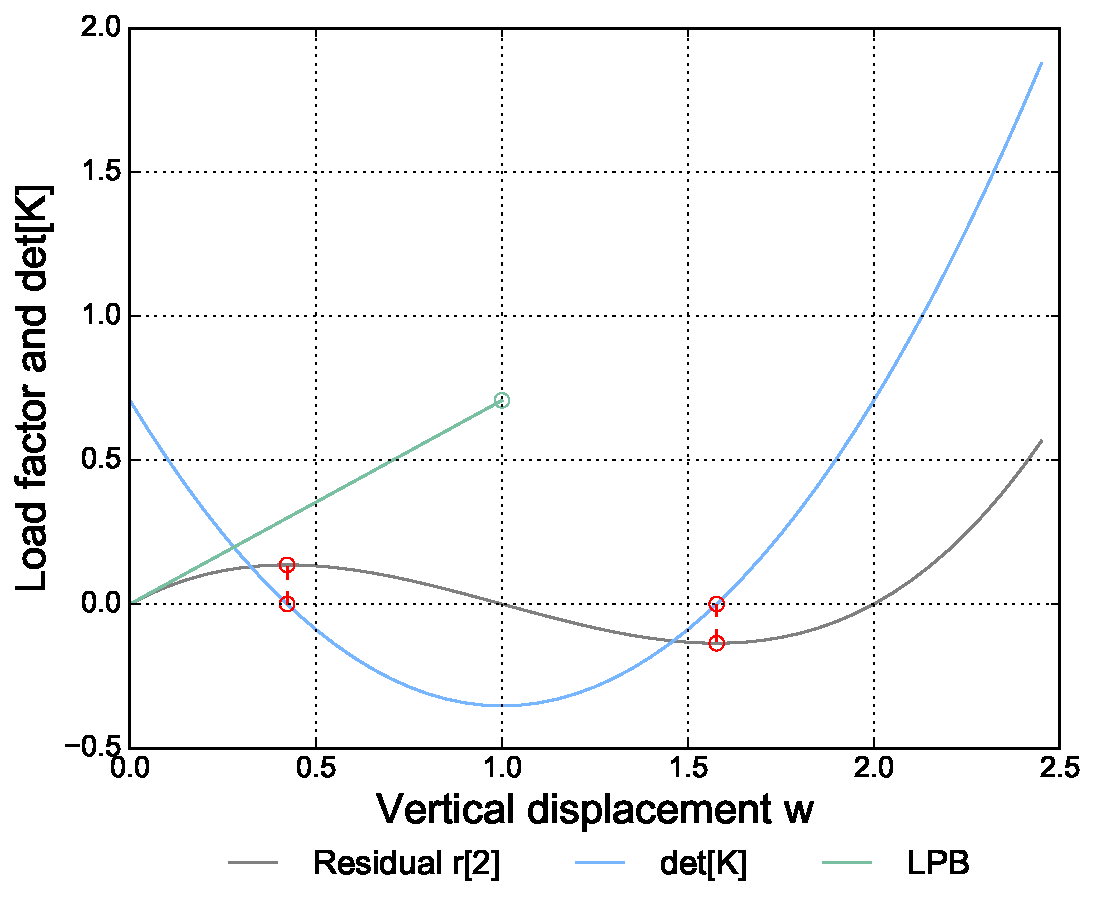
\includegraphics[width=10cm]{images/stability_analysis_mises_truss_1x1.pdf}
	\caption{Ratio of Mises truss LPB and NL critical load factors across varying geometry}
	\label{stab2}
\end{figure}

From the graph it can be seen that the primary equilibrium path traces the two bars snapping through, with $w=1.0$ signifying the bars in a perfectly horizontal position and $w=2.0$ corresponding to a fully snapped through system. Both non-linear critical points are highlighted on the equilibrium path with their connection to the vanishing stiffness determinant at these points explicitly drawn.

As previously discussed, inaccuracies of the LPB analysis are attributable to the consequential pre-critical deflections of the structure. The sensitivity of LPB analysis to this effect can be investigated by gradually increasing the height $b$ of the structure while retaining the same span $a$. As the height over span ratio $b/a$ increases, the structure will become stiffer and pre-critical vertical displacements will reduce. As the actual structural behaviour gradually aligns with the underpinning LPB assumptions, the LPB results should become more accurate. Across the range of $1 \le b/a \le 5$, the ratios of critical LPB load factors to the lowest non-linear critical load factors have been plot in the following figure. Although it is acknowledged that as $b/a$ increase the instability mode will change from a limit to bifurcation point, the detail of interest here is the load factor associated with the onset of instability, regardless of it's nature.

\begin{figure}[H]
	\centering
	\def\svgwidth{\columnwidth}
	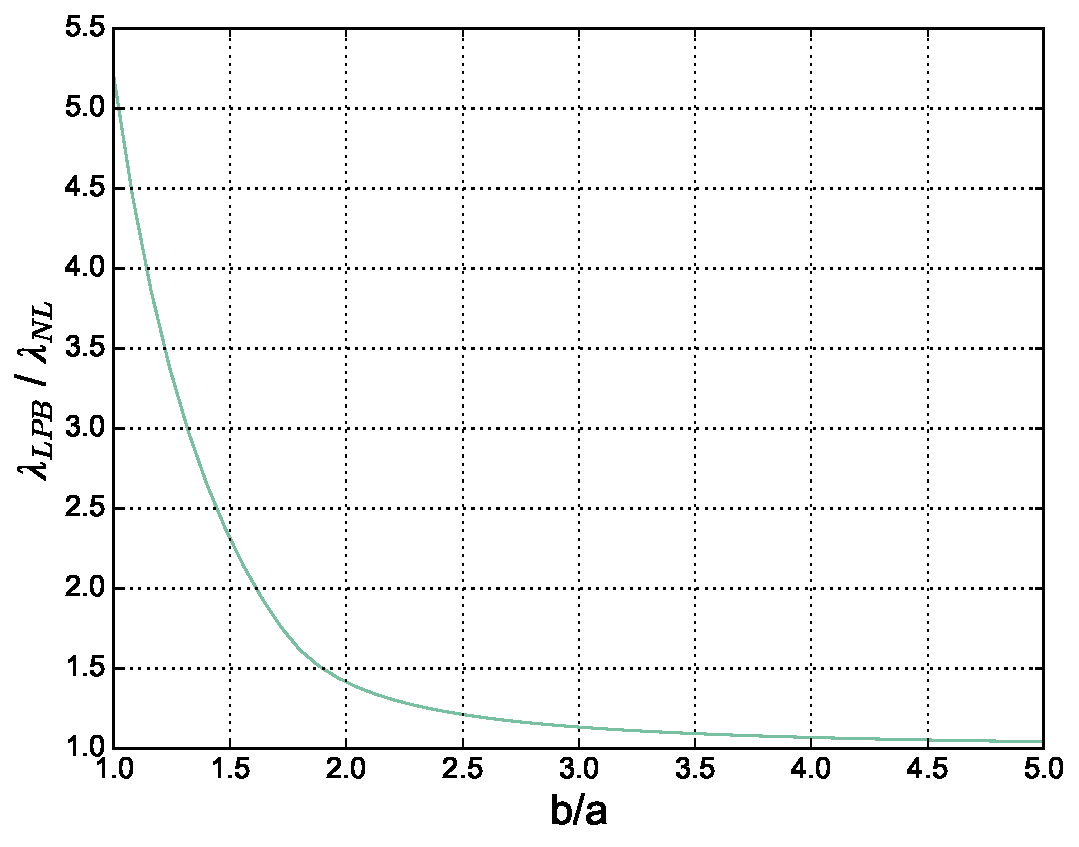
\includegraphics[width=10cm]{images/stability_analysis_mises_truss_lpb.pdf}
	\caption{Ratio of Mises truss LPB and NL critical load factors across varying geometry}
	\label{stab3}
\end{figure}

Consistent with the previous rationale, the LPB analyses tend toward more accurate results as the structure becomes stiffer at greater $b/a$ and pre-critical displacements approach negligible values. Despite this, the figure also confirms that LPB analyses continue to typically overestimate the critical load for a structure. Summarising, it can be seen that when the LPB assumptions are nearly fulfilled it produces quite accurate results with a fraction of computational effort compared to a full non-linear stability analysis, although the tendency to overestimate the onset of instability should also be considered. 

\section{Co-rotational transformation approach - REVIEWED 0}
The Mises truss example highlights that, although the computationally efficient LPB method is accurate for a subset of scenarios, the general case requires fully non-linear analysis. This concept can be extended to general structural analysis employing shell elements, with linear approaches only suitable for a certain subspace of problems. The industrial practical demands of shell elements can be condensed to delivering accurate general solutions in a timely manner. By surveying the typical approaches of commercial FEM packages, the latter point of computational speed is usually fulfilled by employing commonplace shell formulations with linearized strains, however, this seemingly betrays the former requirement of accurate general solutions; one case being problems involving large displacements. A novel solution to this problem, which extends the capability of linear small strain elements to handle large displacements and rotations, is the co-rotational transformation approach.

\subsection{General overview}
The co-rotational (CR henceforth) transformation approach extends the capability of elements normally limited to small strains and  displacements to correctly handle arbitrarily large displacements and rotations, provided strains remain small \cite{FelippaCR1_2016}. Unlike other Lagrangian approaches which 'track' the total displacements via strain only, the CR approach relies upon splitting the total displacements into strain-free rigid body motion and deformational motion.

\begin{figure}[H]
	\centering
	\def\svgwidth{\columnwidth}
	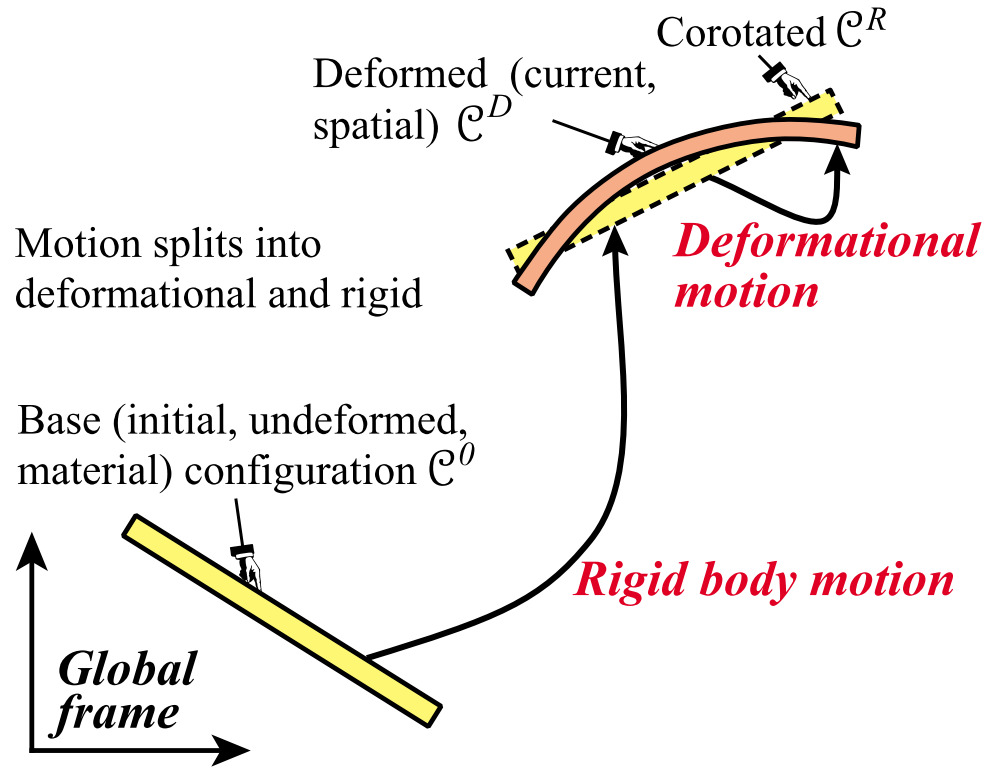
\includegraphics[width=10cm]{images/cr_1.png}
	\caption{CR kinematic description \cite{FelippaCR1_2016}}
	\label{cr1}
\end{figure}

The above figure illustrates this division of total displacement by way of a simple beam example. The base configuration $\mathscr{C}^0$ evidently refers to the initial un-deformed state of the element. The co-rotated configuration $\mathscr{C}^R$, also called the shadow configuration, is the frame arrived at by extracting the rigid body motion of the element's total displacement. If the remaining deformational motion is applied to state $\mathscr{C}^R$ the final deformed configuration $\mathscr{C}^D$ is achieved. Although the CR approach reduces the deformation motion experienced by the element, which will mechanically respond according to it's formulation, the process of reducing this deformation motion via filtering out rigid body motion is independent of the element's formulation. Thus, the scope of CR discussion henceforth is focussed on the element-independent CR (EICR) formulation.

\section{EICR formulation overview - REVIEWED 0 !!!!!}
The EICR, owing to it's name and as previously described, is a CR approach independent of the element formulation. Because of this element formulation independence it allows re-use of linear elements in a non-linear context, provided small strain assumptions aren't violated. Thus, the EICR can also be interpreted as a geometric-based filter stripping away rigid body motion from the deformations seen by each element. The following flowchart illustrates the general function of the EICR in a typical FEM program.

\begin{figure}[H]
	\centering
	\def\svgwidth{\columnwidth}
	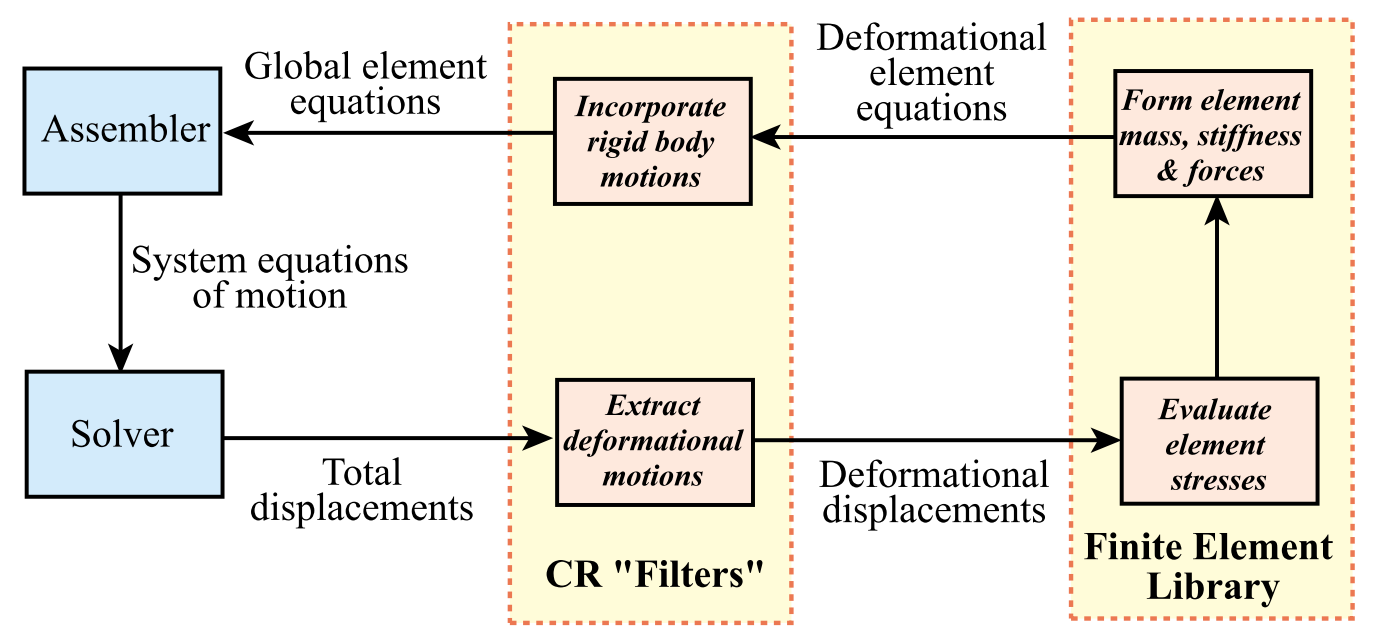
\includegraphics[width=14cm]{images/cr_3.png}
	\caption{EICR scheme \cite{FelippaCR1_2016}}
	\label{cr3}
\end{figure}

Two key components of the EICR formulation corresponding with the CR blocks above are: extracting the deformational motions by means of EICR kinematics before element computation; and the incorporation of rigid body motions into the calculated element tangent stiffness. These two EICR components are considered in the following subsections.

\subsection{EICR kinematics}
An overview of the EICR kinematics utilised to separate total element displacements into rigid body motion and deformational motion is henceforth described. Only a high level functional overview of the formulation components is contained herein, for a full treatment of the topic the reader may refer to selected works of Felippa (References \cite{FelippaCR1_2016}) and \cite{felippa2000systematic}) and Haugen's PhD thesis (Reference \cite{Hau94}). The following figure illustrates an element in various states of the EICR transformation:

\begin{figure}[H]
	\centering
	\def\svgwidth{\columnwidth}
	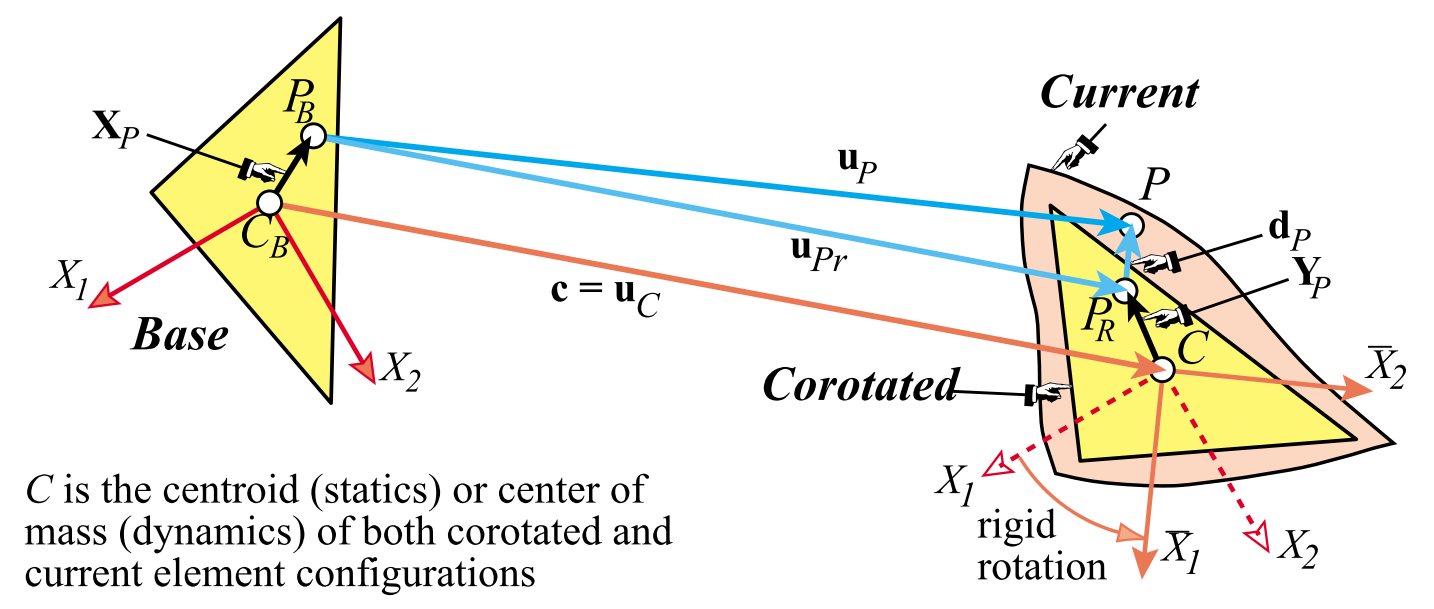
\includegraphics[width=14cm]{images/cr_4.png}
	\caption{Kinematics of co-rotated element \cite{felippa2000systematic}}
	\label{cr4}
\end{figure}

The base state $\mathscr{C}^0$ displays quantities such as it's centroid $C_B$, local axes $X_1$ and $X_2$ and the position vector $\mathbf{X}_P$ of an arbitrary point $P_B$. Moving to the co-rotated frame $\mathscr{C}^R$, it's centroid is denoted $C$, with $\mathbf{Y}_P$ denoting the position vector of the transformed original base point $P_B$ expressed in the co-rotated frame as $P_R$. The original $\mathscr{C}^0$ axes $X_1$ and $X_2$ are shown along with their co-rotated counterparts $\bar{X}_1$ and $\bar{X}_2$. Vector $\mathbf{u}_P$ defines the total displacement of point $P_B$ which can be decomposed into rigid body $\mathbf{u}_{Pr}$ and deformational motion $\mathbf{d}_p$ according to:

\begin{equation} 
\mathbf{u}_P = 
\mathbf{u}_{Pr} + \mathbf{d}_p
\label{eq_cr1}\ .
\end{equation}

The rigid body motion $\mathbf{u}_{Pr}$ itself can be decomposed into rigid body translation of the element centroid $\mathbf{u}_c$ and rigid body rotation of $\mathbf{X}_P$ to $\mathbf{Y}_P = \mathbf{R} \mathbf{X}_P$ via the orthogonal rotation matrix $\mathbf{R}$ (described below). If point $P$ position vectors $\mathbf{X}_P$ and $\mathbf{Y}_P$ are included in equation \ref{eq_cr1}, one can write:

\begin{equation} 
\mathbf{u}_P + \mathbf{X}_P = 
\mathbf{u}_{c} + \mathbf{d}_p + \mathbf{Y}_P
\label{eq_cr2}\ .
\end{equation}

The deformational motion $\mathbf{d}_p$ can be extracted in $\mathscr{C}^0$ by rearranging the above equation and substituting the relation $\mathbf{Y}_P = \mathbf{R} \mathbf{X}_P$ yielding:

\begin{equation} 
\mathbf{d}_p = 
\mathbf{u}_P - \mathbf{u}_{c} - (\mathbf{R} - \mathbf{I}) \mathbf{X}_P 
\label{eq_cr3}\ .
\end{equation}

As per the general flow of figure \ref{cr3}, the deformational motion described above form the totality of displacements 'seen' by the element. Since these displacements, and the element stiffness matrix and internal force vector computed via virtual displacements $\delta \mathbf{v}$, are computed in $\mathscr{C}^R$, the variation of these in $\mathscr{C}^R$ require additional treatment to be linked back to the global frame. This additional workload corresponds to the upper EICR block of figure \ref{cr3}, with the treatment of EICR internal forces considered first.

\subsection{EICR internal forces}
The element internal force vector $\mathbf{p}_R^e$ in the CR frame $\mathscr{C}^R$ for each node $a = 1\ ...\ N^e$ is given by the internal energy $U^e$ derived through it's DOFs:

\begin{equation} 
\mathbf{p}_R^e = 
\frac{\partial U^e}{\partial \mathbf{v}_R^e}
\label{eq_cr4}\ ,
\end{equation}

which can be split into translation and moment forces as per:

\begin{equation} 
\mathbf{p}_R^e = 
\begin{pmatrix}
\mathbf{p}_{Ru}^e \\
\mathbf{p}_{R\theta}^e 
\end{pmatrix}
=
\begin{pmatrix}
\frac{\partial U^e}{\partial \mathbf{u}_{R}^e} \\
\frac{\partial U^e}{\partial \boldsymbol{\theta}_{R}^e} 
\end{pmatrix}
\label{eq_cr5}\ .
\end{equation}

With a view of reconciling the above expressions in the global frame variations in the CR configuration $\mathscr{C}^R$ $\delta \mathbf{u}_{R}^e,\ \delta \boldsymbol{\theta}_{R}^e$ must be related back to the global frame $\delta \mathbf{u}^e,\ \delta \boldsymbol{\omega}^e$ via the Jacobian $\mathbf{J}$:

\begin{equation} 
\begin{pmatrix}
\delta \mathbf{u}_{R}^e \\
\delta \boldsymbol{\theta}_{R}^e
\end{pmatrix}
=
\mathbf{J}
\begin{pmatrix}
\delta \mathbf{u}^e \\
\delta \boldsymbol{\omega}^e
\end{pmatrix}\ ,
\hspace{10mm}
\mathbf{J} = 
\begin{pmatrix}
\frac{\partial \mathbf{u}_R^e}{\partial \mathbf{u}^e} & \frac{\partial \mathbf{u}_R^e}{\partial \boldsymbol{\omega}^e} \\
\frac{\partial \boldsymbol{\theta}_R^e}{\partial \mathbf{u}^e} & \frac{\partial \boldsymbol{\theta}_R^e}{\partial \boldsymbol{\omega}^e}
\end{pmatrix}
\label{eq_cr6}\ .
\end{equation}

Key to the EICR is that energy scalars between various configurations $\mathscr{C}$ shouldn't change. Thus, if one considers internal virtual work in terms of the internal force vector between global and $\mathscr{C}^R$ frames the following equality must hold:

\begin{equation} 
(\mathbf{p}_{Ru}^{e})^T  \delta \mathbf{u}_{R}^e +
(\mathbf{p}_{R\theta}^{e})^T \delta \boldsymbol{\theta}_{R}^e =
(\mathbf{p}_{u}^{e})^T  \delta \mathbf{u}_{}^e +
(\mathbf{p}_{\theta}^{e})^T \delta \boldsymbol{\theta}_{}^e
\label{eq_cr7}\ ,
\end{equation}
with the transformed global internal forces determined as:
\begin{equation} 
\begin{pmatrix}
\mathbf{p}_{u}^e \\
\mathbf{p}_{\theta}^e 
\end{pmatrix}
=
\mathbf{J}^T
\begin{pmatrix}
\mathbf{p}_{Ru}^e \\
\mathbf{p}_{R\theta}^e 
\end{pmatrix}
\label{eq_cr8}\ .
\end{equation}

Felippa proposes in Reference \cite{felippa2005unified} that it is convenient to split the Jacobian matrix up into the following components:

\begin{equation} 
\mathbf{J}
= \mathbf{H}_R 
\mathbf{P}_R 
\mathbf{T}
\label{eq_cr9}\ .
\end{equation}

Exact expressions for determining the matrices introduced above can be found in References \cite{felippa2005unified}, \cite{felippa2000systematic} and \cite{FelippaCR1_2016}. For the purposes of this EICR overview functional descriptions are provided below \cite{felippa2005unified}:

\begin{itemize}
	\item $\mathbf{H}$ = Jacobian derivative of the (global) rotational axial vector $\boldsymbol{\theta}$ with respect to the ($\mathscr{C}^R$) spin axial vector $\boldsymbol{\theta}$.
	\item $\mathbf{P}$ = Projector matrix which preserves deformational motion from total displacements by projecting out rigid body motion.
	\item $\mathbf{T}$ = Global-to-local transformation matrix such that $\mathbf{u}_R = \mathbf{T} \mathbf{u}$.
\end{itemize}

Summarising, the movement from global to $\mathscr{C}^R$ DOF variations is succinctly distilled in the following figure:

\begin{figure}[H]
	\centering
	\def\svgwidth{\columnwidth}
	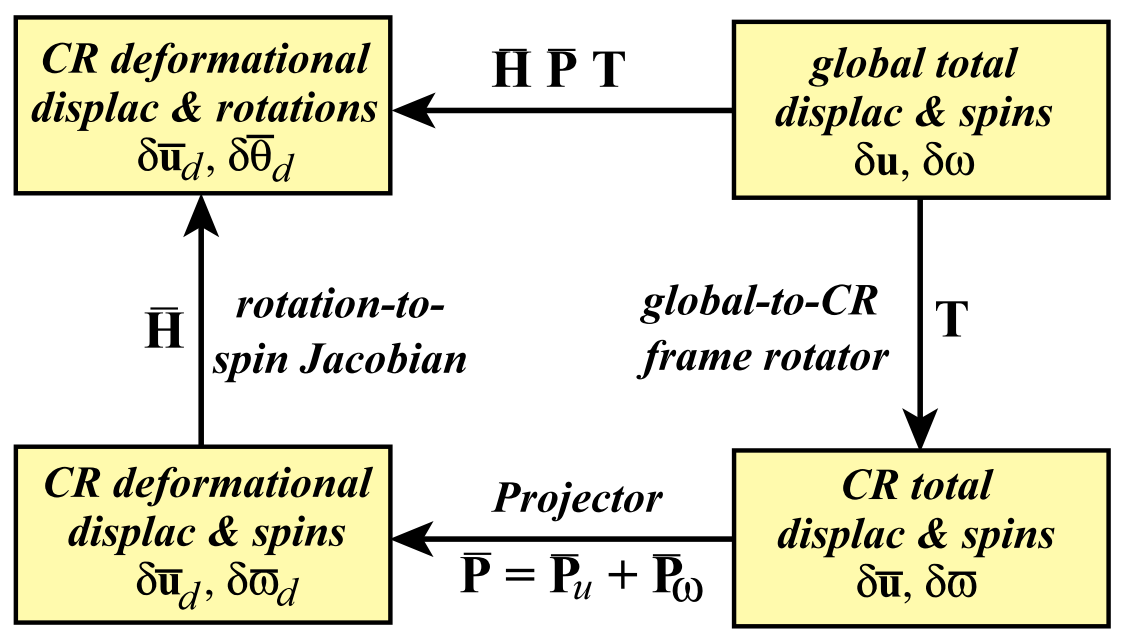
\includegraphics[width=10cm]{images/cr_6.png}
	\caption{Movement from global to CR frames \cite{felippa2005unified}}
	\label{cr6}
\end{figure}

Reversing the direction of movement (from $\mathscr{C}^R$ to global frames) is achieved as per equation \ref{eq_cr8}, with $\mathbf{J}^T = \mathbf{T}^T \mathbf{P}_R^T \mathbf{H}_R^T$. Thus, the global internal force vector $\mathbf{p}^e$ can be recovered according to:

\begin{equation} 
\mathbf{p}^e
=
\mathbf{T}^T \mathbf{P}_R^T \mathbf{H}_R^T
\mathbf{p}_R^e
\label{eq_cr10}\ .
\end{equation}
 
 \subsection{EICR tangent stiffness}
 Just as the internal force vector must be transformed from the $\mathscr{C}^R$ to the global frame, so must the element tangent stiffness computed in $\mathscr{C}^R$. Felippa defines the consistent tangent stiffness $\mathbf{K}^e$ of element $e$ as the variation of internal forces with respect to element DOFs \cite{felippa2005unified}; mathematically:
 
 \begin{equation} 
\delta \mathbf{p}^e
 =
\mathbf{K}^e \delta \mathbf{v}^e\ ,
\hspace{5mm}
with
\hspace{5mm}
\mathbf{K}^e = 
\frac{\partial \mathbf{p}^e}{\partial \mathbf{v}^e}
 \label{eq_cr11}\ .
 \end{equation}
 
 If the variation of $\mathbf{p}^e$ is taken in equation \ref{eq_cr10}, the chain rule arises 4 times yielding:
 
  \begin{equation} 
 \delta \mathbf{p}^e
 =
\delta \mathbf{T}^T \mathbf{P}_R^T \mathbf{H}_R^T \mathbf{p}_R^e
+
\mathbf{T}^T \delta \mathbf{P}_R^T \mathbf{H}_R^T \mathbf{p}_R^e
+
\mathbf{T}^T \mathbf{P}_R^T \delta \mathbf{H}_R^T \mathbf{p}_R^e
+
\mathbf{T}^T\mathbf{P}_R^T \mathbf{H}_R^T  \delta \mathbf{p}_R^e
 \label{eq_cr12}\ ,
 \end{equation}
 
 condensing terms together yields:
 
   \begin{equation} 
 \delta \mathbf{p}^e
 =
(\mathbf{K}_{GR}^e + 
\mathbf{K}_{GP}^e + 
\mathbf{K}_{GM}^e + 
\mathbf{K}_{M}^e
)
\delta \mathbf{v}^e
 \label{eq_cr13}\ .
 \end{equation}
 
 The introduced terms above can be identified as stiffness contributions transformed from $\mathscr{C}^R$ to the global frame:
 
 \begin{itemize}
 	\item $\mathbf{K}_{GR}^e$ = Rotational-correction geometric stiffness.
 	\item $\mathbf{K}_{GP}^e$ = Equilibrium projection geometric stiffness.
 	\item $\mathbf{K}_{GM}^e$ = Moment-correction geometric stiffness.
 	\item $\mathbf{K}_{M}^e$ = Material stiffness.
 \end{itemize}
 
 Detailed standalone expressions of the above contributions can be found in Felippa's works \cite{felippa2005unified}, \cite{felippa2000systematic} and \cite{FelippaCR1_2016} and fall outside the scope of this overview. Development and combination of these expressions leads to the complete form of the element tangent stiffness in the global frame \cite{felippa2005unified}:
 
\begin{equation} 
\mathbf{K}^e 
 =
 \mathbf{T}^T
 (
 \mathbf{P}_R^T
 \mathbf{H}_R^T
 \mathbf{K}_R^e
  \mathbf{H}_R
   \mathbf{P}_R
+
 \mathbf{P}_R^T
  \mathbf{L}_R
\mathbf{P}_R
-
\mathbf{F}_{RNM}
 \mathbf{G}_R
 -
  \mathbf{G}_R^T
  \mathbf{F}_{RN}^T
\mathbf{P}_R
 )
\mathbf{T}
 \label{eq_cr14}\ .
 \end{equation}
 
 Full derivations of the terms $\mathbf{L}_R$ (spin derivative of $\mathbf{H}$ contracted with nodal moments), $\mathbf{G}_R$ (spin-fitter linking variations in $\mathscr{C}^R$ element-centroid spin with nodal DOFs), $\mathbf{F}_{RNM}$ (spin of nodal forces and moments) and $\mathbf{F}_{RN}$ (spin of nodal forces) can be found in Reference \cite{felippa2005unified}. Of more relevance to this overview are the simplifications available to the complete element tangent stiffness above which form 3 hierarchical formulations, summarised in ascending order of accuracy.
 
  \begin{itemize}
 	\item EICR tangent stiffness: consistent CR formulation (C):
 	\begin{itemize}
 		\item $\mathbf{K}^e 
 		=
 		\mathbf{T}^T
 		(
 		\mathbf{K}_R^e
 		\mathbf{H}_R
 		\mathbf{P}_R
 		-
 		\mathbf{F}_{RNM}
 		\mathbf{G}_R
 		)
 		\mathbf{T}$
		\item Reduction to material and rotational geometric stiffness terms.
		\item Material stiffness approaches symmetry with refining element mesh if the membrane strains are small.
 		\item Unsymmetric element geometric stiffness matrix.
 		\item Unsymmetric global stiffness matrix, loss of quadratic convergence.
 	\end{itemize}
 	\item EICR tangent stiffness: consistent equilibrated CR formulation (CE):
 	\begin{itemize}
 		\item $\mathbf{K}^e 
 		=
 		\mathbf{T}^T
 		(
 		\mathbf{P}_R^T
 		\mathbf{K}_R^e
 		\mathbf{H}_R
 		\mathbf{P}_R
 		-
 		\mathbf{F}_{RNM}
 		\mathbf{G}_R
 		-
 		\mathbf{G}_R^T
 		\mathbf{F}_{RN}^T
 		\mathbf{P}_R
 		)
 		\mathbf{T}$
 		\item Addition of projector $\mathbf{P}_R$ to (C) formulation.
 		\item Material stiffness approaches symmetry with refining element mesh.
 		\item Unsymmetric element geometric stiffness matrix.
 		\item Symmetric global stiffness matrix (provided there are no nodal moments), quadratic convergence achieved.
 	\end{itemize}
 	\item EICR tangent stiffness: consistent symmetrizable equilibrated CR formulation (CSE):
 		\begin{itemize}
 		\item $\mathbf{K}^e 
 		=
 		\mathbf{T}^T
 		(
 		\mathbf{P}_R^T
 		\mathbf{H}_R^T
 		\mathbf{K}_R^e
 		\mathbf{H}_R
 		\mathbf{P}_R
 		+
 		\mathbf{P}_R^T
 		\mathbf{L}_R
 		\mathbf{P}_R
 		-
 		\mathbf{F}_{RNM}
 		\mathbf{G}_R
 		-
 		\mathbf{G}_R^T
 		\mathbf{F}_{RN}^T
 		\mathbf{P}_R
 		)
 		\mathbf{T}$
 		\item All terms of equation \ref{eq_cr14} retained. 
 		\item Material stiffness is always symmetric.
 		\item Unsymmetric element geometric stiffness matrix.
 		\item Symmetric global stiffness matrix (provided there are no nodal moments), quadratic convergence achieved.
 	\end{itemize}
 \end{itemize}

The hierarchical formulations demonstrate that the simplifying assumptions in the C and CE formulations introduce limitations when compared to the full CSE. Currently the CE EICR formulation is implemented in Kratos providing a reasonable balance between practical accuracy and computational speed. Utilising this formulation, existing Kratos linear small strain shell elements have been proven capable of accurate geometrically non-linear analysis.

\section{Chapter summary - TO DO !!!!!!!!!!!!!!!!}
